\documentclass[11pt,a4paper]{article}
\usepackage[utf8]{inputenc}
\usepackage{amsmath,amsfonts,amssymb}
\usepackage{graphicx}
\usepackage{geometry}
\geometry{margin=1in}
\usepackage{booktabs}
\usepackage{hyperref}
\usepackage{float}
\usepackage{xcolor}

\title{\textbf{EE3621: Digital Signal Processing} \\ \Large Lecture 27: DSP for Image Processing — 2D DFT, Filtering \& Transforms \\ \large (III B.Tech EEE)}
\author{Lecture Notes (40-Minute Plan)}
\date{}

\definecolor{darkbg}{HTML}{0d121f}
\definecolor{lighttext}{HTML}{e2e8f0}
\definecolor{primary}{HTML}{8b5cf6}
\definecolor{secondary}{HTML}{0dd5c5}

\pagecolor{darkbg}
\color{lighttext}

\hypersetup{
    colorlinks=true,
    linkcolor=secondary,
    urlcolor=secondary
}

\begin{document}

\maketitle

\section{Lecture Plan (40 Minutes Breakdown)}
\begin{itemize}
    \item \textbf{00:00 -- 05:00 (5 mins):} Welcome \& 2D Signals. Introduction to digital images, spatial sampling, and aliasing.
    \item \textbf{05:00 -- 12:00 (7 mins):} 2D DTFT and 2D DFT. Spatial frequency spectrum, separability, and row-column FFT computations.
    \item \textbf{12:00 -- 18:00 (6 mins):} 2D Convolution \& Filtering. Derivations of separability and computational savings.
    \item \textbf{18:00 -- 24:00 (6 mins):} Spatial Frequency Domain Filtering. Low-pass vs.\ High-pass, Gaussian, and Laplacian.
    \item \textbf{24:00 -- 30:00 (6 mins):} 2D Discrete Cosine Transform (DCT). Energy compaction and JPEG block-level processing.
    \item \textbf{30:00 -- 36:00 (6 mins):} Edge Detection. Gradient operators (Sobel), gradient magnitude/direction, and Canny steps.
    \item \textbf{36:00 -- 40:00 (4 mins):} Summary, Key Formulas, and Checkpoint Questions.
\end{itemize}

\noindent\rule{\textwidth}{0.5pt}

\section{2D Signals: The Digital Image}

\begin{figure}[H]
    \centering
    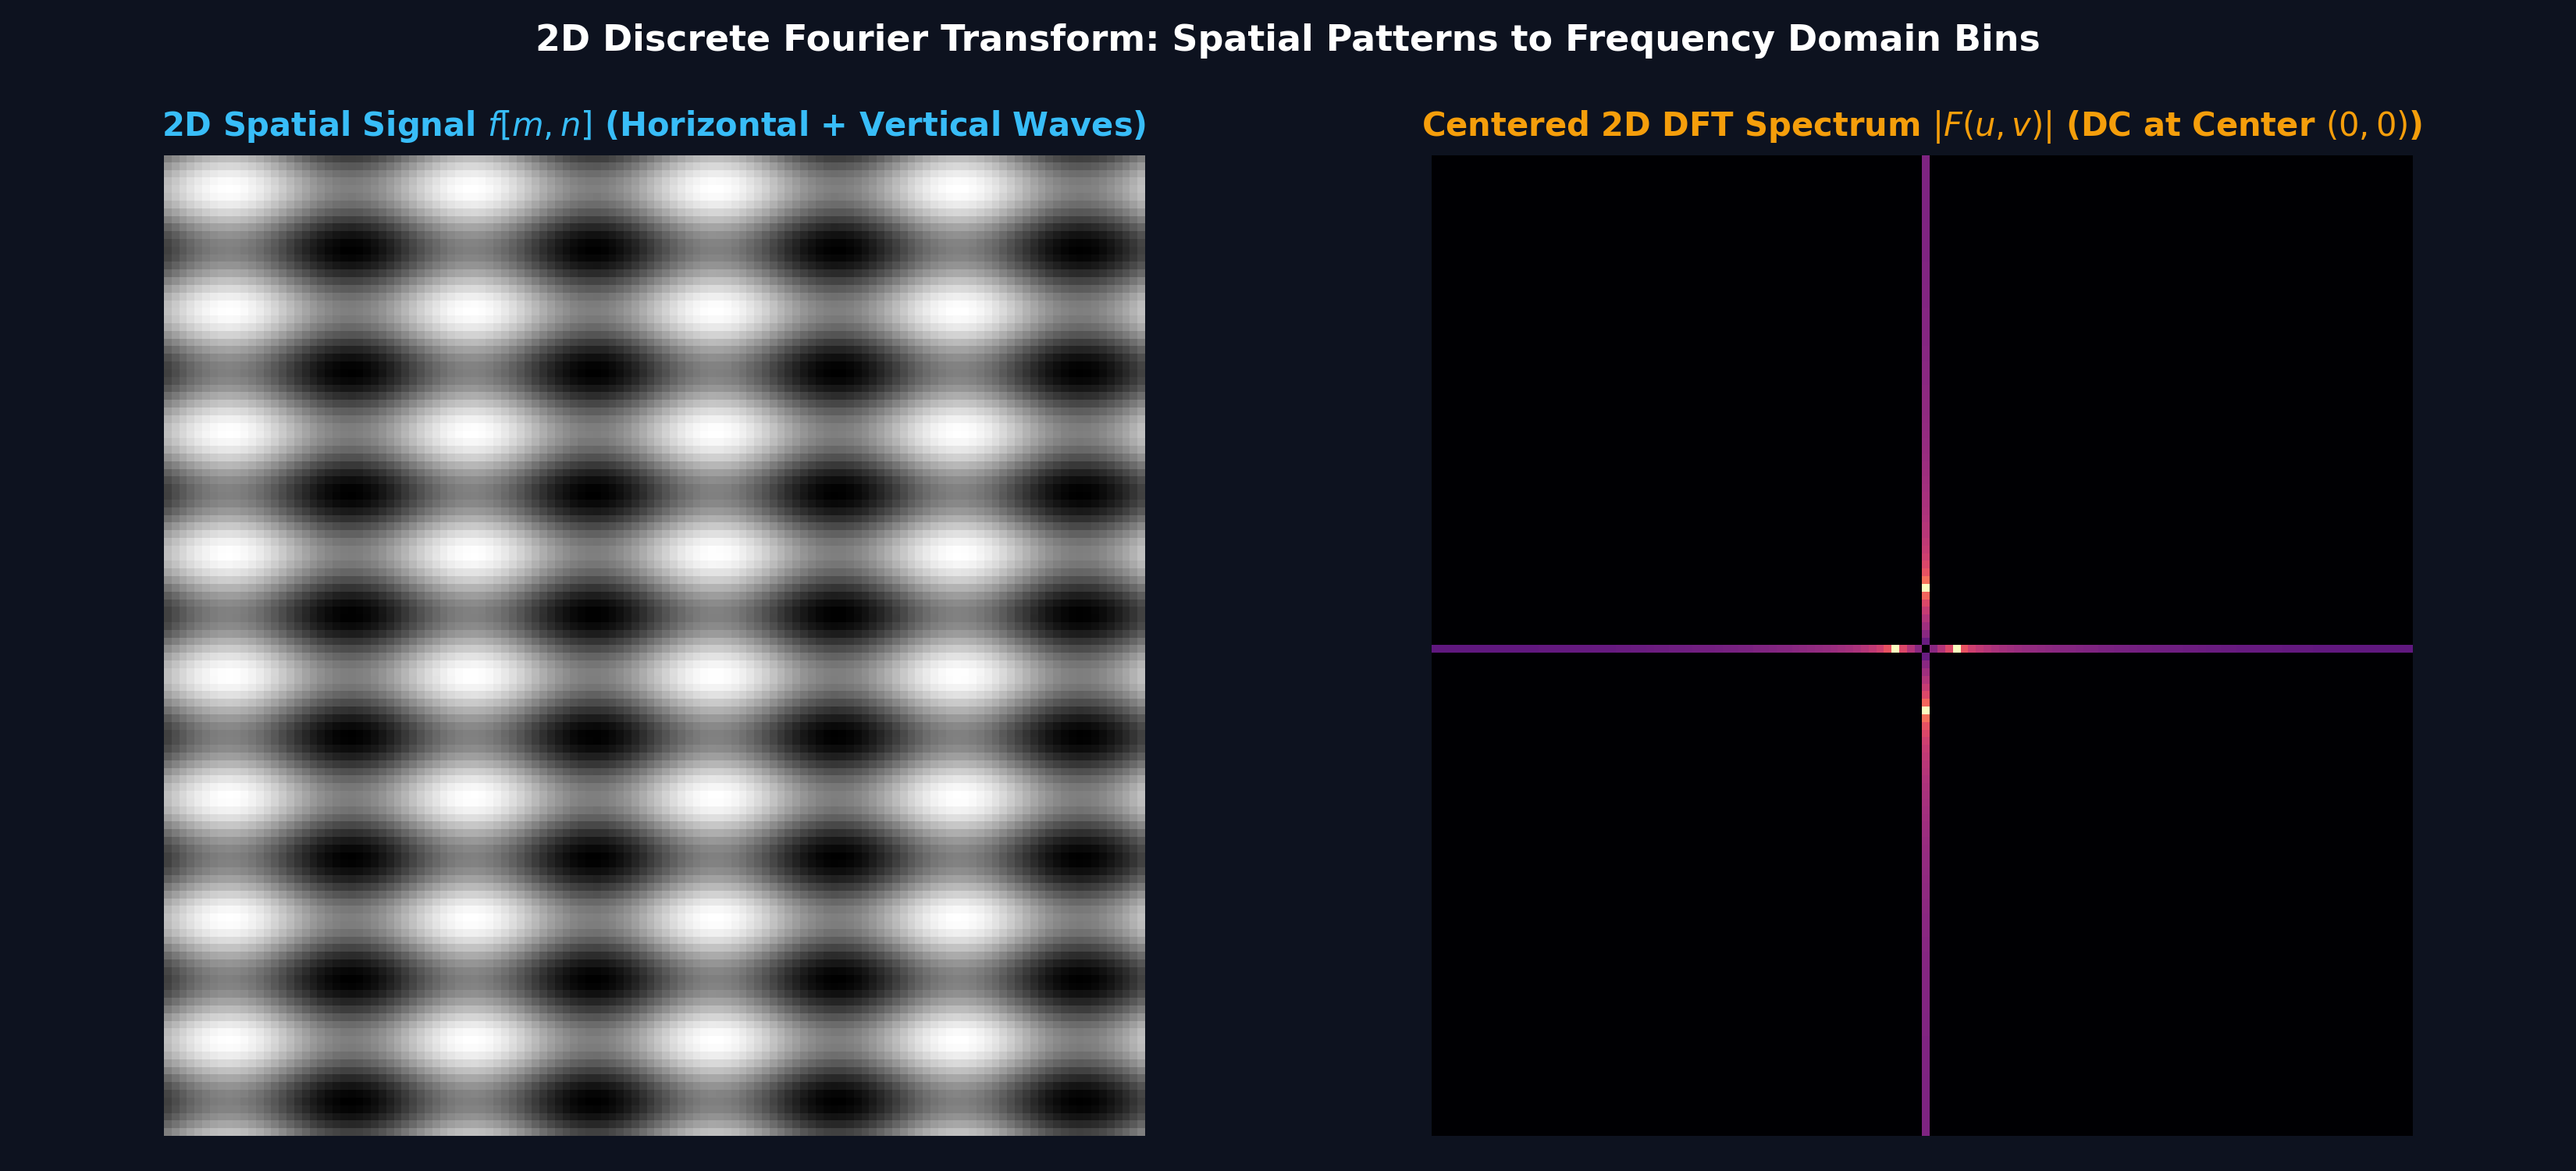
\includegraphics[width=0.85\textwidth]{images/image_2d_dft_spatial_frequencies.png}
    \caption{2D Discrete Fourier Transform: Mapping Spatial Image Brightness Patterns to Frequency Coordinates.}
\end{figure}

\begin{figure}[H]
    \centering
    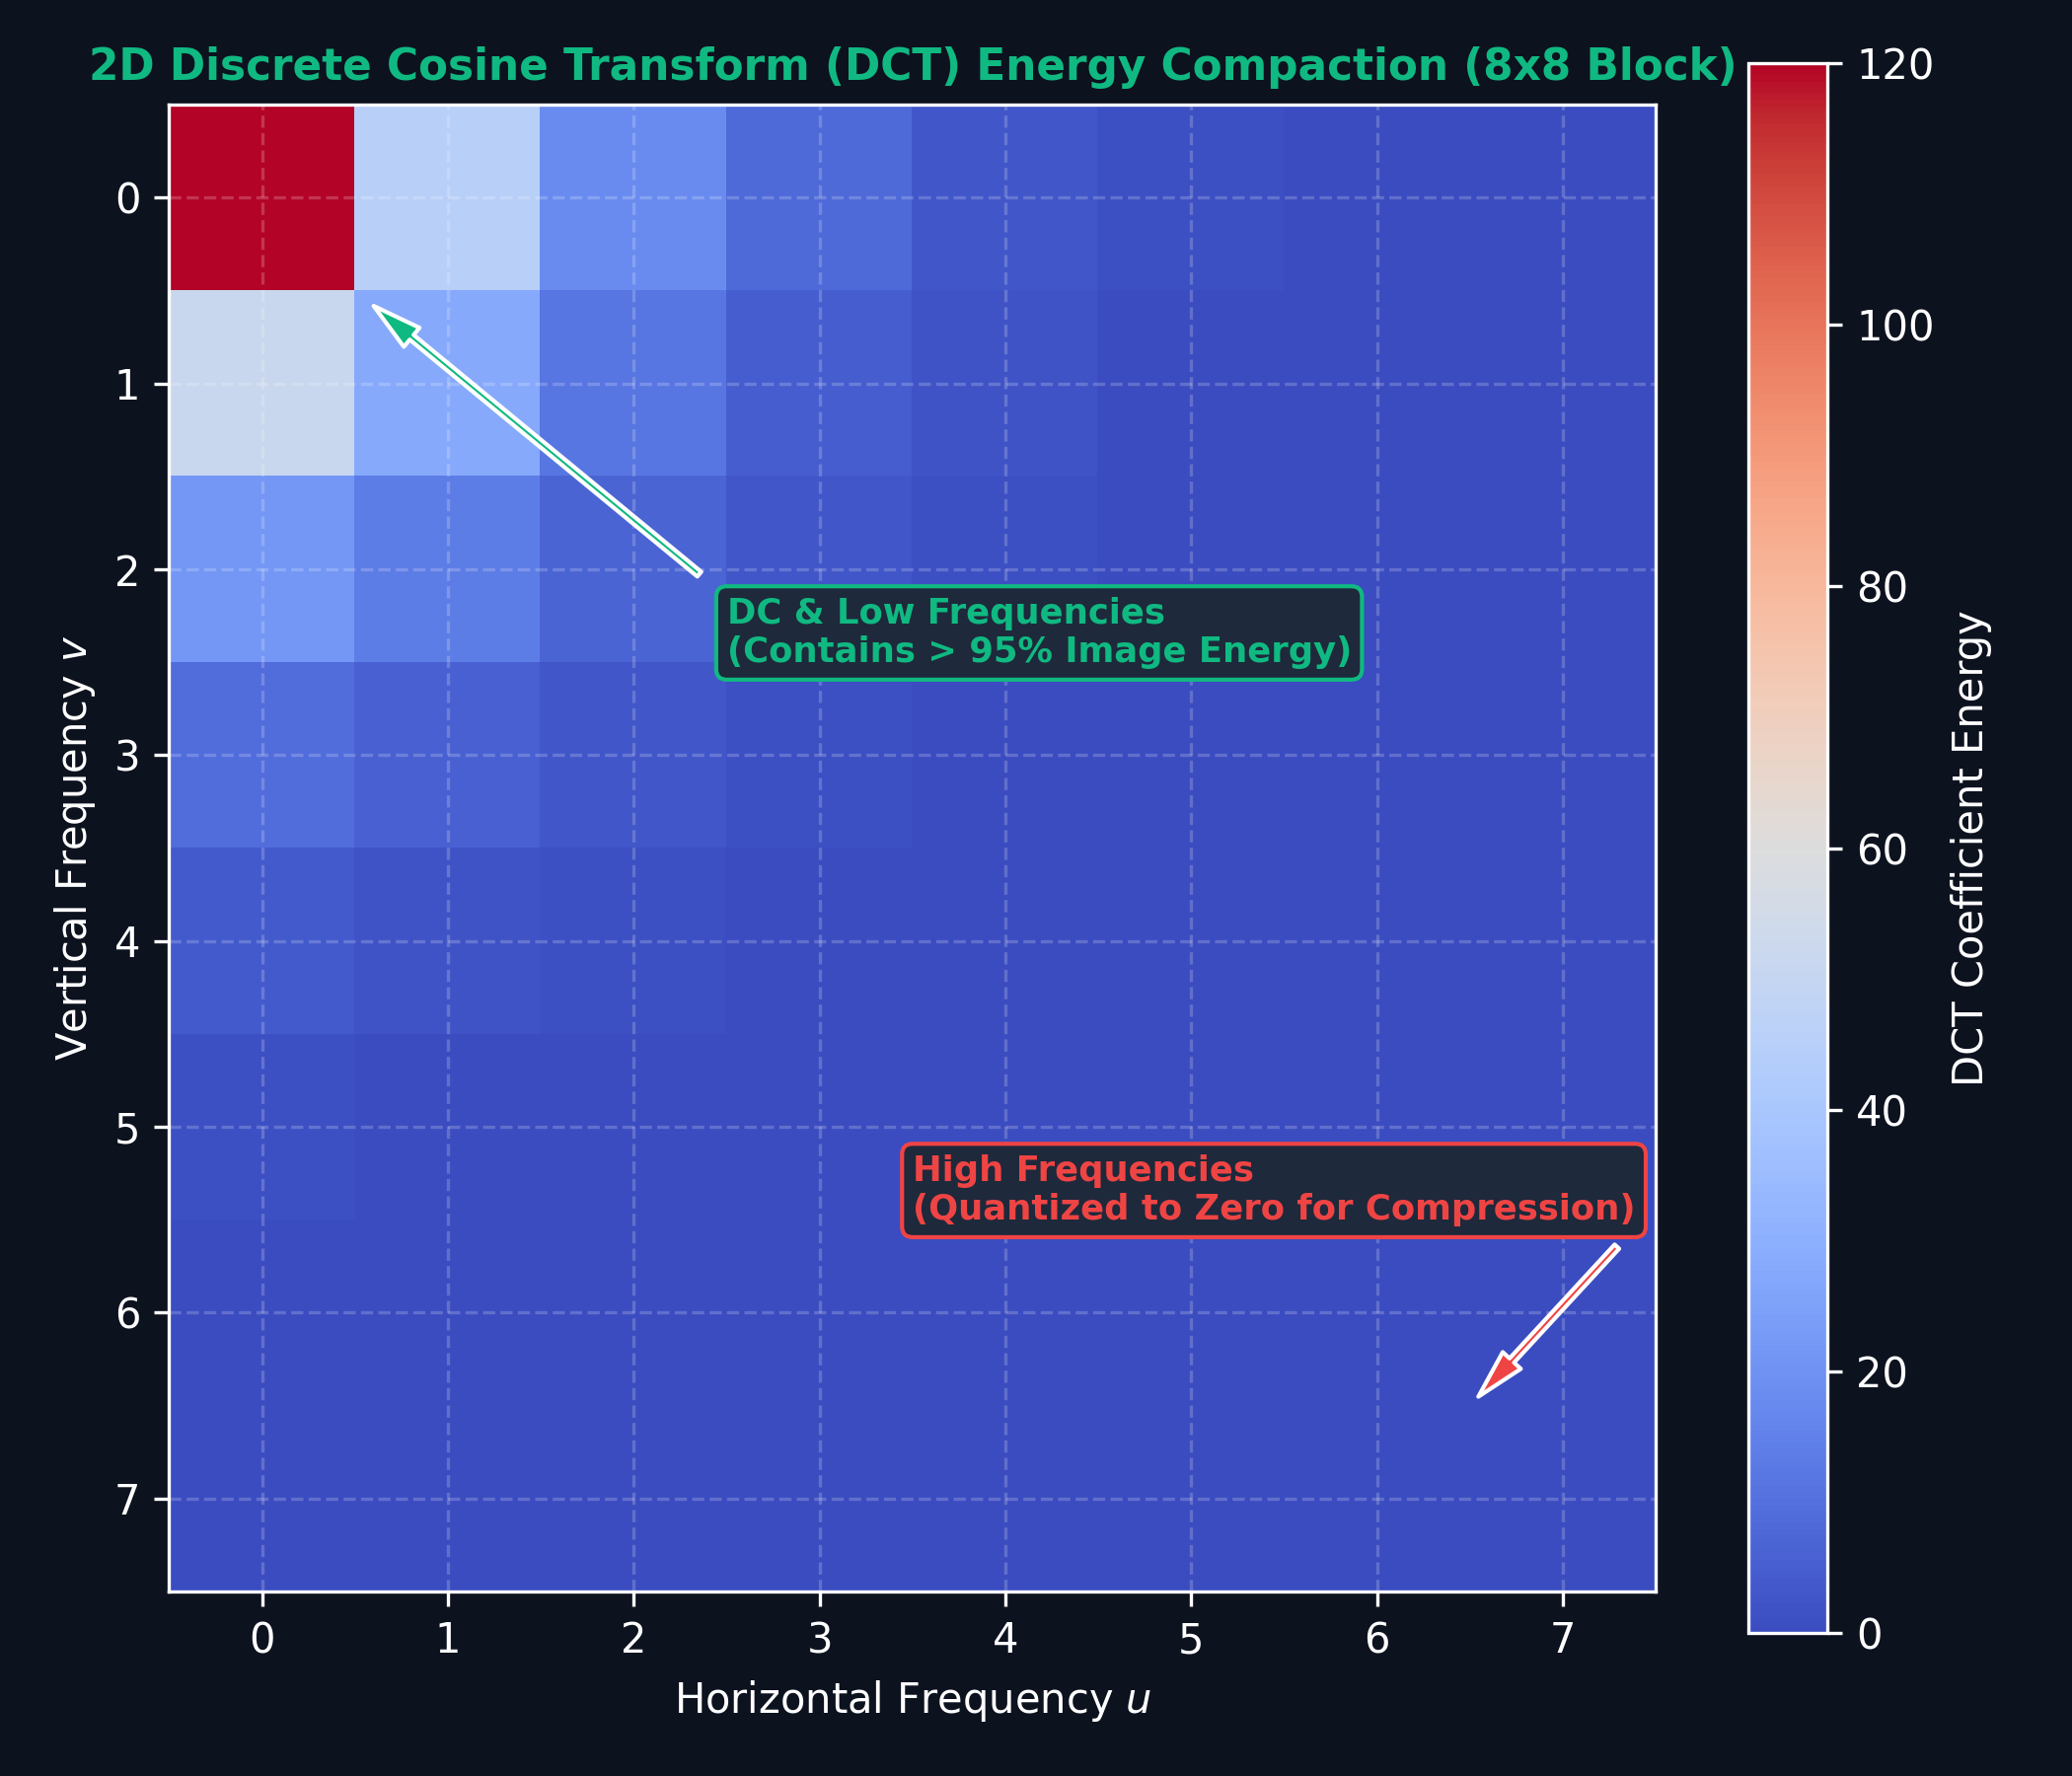
\includegraphics[width=0.65\textwidth]{images/jpeg_2d_dct_energy_compaction.png}
    \caption{2D Discrete Cosine Transform (DCT) Energy Compaction Matrix in $8\times 8$ JPEG Compression.}
\end{figure}


In traditional 1D digital signal processing, a signal $x[n]$ is typically a sequence of values indexed by time (e.g., an audio recording). In the realm of image processing, however, a digital image is fundamentally a \textbf{2D discrete signal}, denoted by $f[m,n]$. Here, $m$ and $n$ are discrete spatial coordinates representing the rows and columns of a pixel grid.

\subsection{Pixel Values and Domains}
When we sample an optical image, we discretize both the spatial coordinates and the amplitude (intensity) of the light.
\begin{itemize}
    \item \textbf{Grayscale Images:} The function $f[m,n]$ represents a single intensity value for each coordinate pair. This is typically mapped on an 8-bit scale, ranging from $0$ (pure black) to $255$ (pure white). Intermediate values represent varying shades of gray.
    \item \textbf{Color Images (RGB):} A color image is a multidimensional signal. Each pixel consists of three separate channels: Red, Green, and Blue. Thus, the image can be viewed as three stacked 2D signals: $f_R[m,n]$, $f_G[m,n]$, and $f_B[m,n]$, or as a single 3D tensor $f[m,n,c]$ where $c \in \{0, 1, 2\}$.
\end{itemize}

\subsection{Spatial Sampling and Aliasing}
Just as a 1D continuous audio signal must be sampled above the Nyquist rate to avoid temporal aliasing (where high frequencies masquerade as low frequencies), a continuous 2D optical image $f_c(x,y)$ must be sampled with an adequately fine spatial resolution. The spatial resolution is determined by the density of the sensor pixels.

\textbf{Physical Intuition:} 
Imagine taking a digital photograph of a brick wall from far away, or a person wearing a shirt with very fine, densely packed stripes. These physical objects represent \textbf{high spatial frequencies} because the visual intensity changes very rapidly over a small spatial distance. 

If your camera's sensor does not have enough pixels to capture these rapid changes (i.e., you are sampling below the spatial Nyquist rate), the high-frequency stripes will fold over into lower frequencies. Visually, this manifests as \textbf{Moiré patterns}—strange, wavy, artificial low-frequency artifacts that do not exist in the real object. 

This is \textbf{spatial aliasing}, which is conceptually identical to the 1D aliasing demonstrated below (from our earlier analysis on frequency folding). Notice how high-frequency spectral components wrap around and corrupt the primary band.

\section{2D DTFT and 2D DFT}
To analyze the frequency content of images—to understand where the rapid changes (edges) and slow changes (smooth areas) lie—we must extend our Fourier analysis tools into two dimensions.

\subsection{The 2D Discrete-Time Fourier Transform (DTFT)}
The 2D DTFT is the theoretical bridge that converts a discrete spatial domain signal $f[m,n]$ of infinite extent into a continuous spatial frequency domain representation, denoted as $F(e^{j\omega_x}, e^{j\omega_y})$:
\begin{equation}
F(e^{j\omega_x}, e^{j\omega_y}) = \sum_{m=-\infty}^{\infty} \sum_{n=-\infty}^{\infty} f[m,n] e^{-j(\omega_x m + \omega_y n)}
\end{equation}

\textbf{Physical Intuition in the Frequency Domain:}
\begin{itemize}
    \item \textbf{$\omega_x$ (Horizontal Frequency):} Represents the rate of variation across the horizontal axis (columns). A high $\omega_x$ means rapid changes horizontally, which corresponds to vertical edges.
    \item \textbf{$\omega_y$ (Vertical Frequency):} Represents the rate of variation down the vertical axis (rows). A high $\omega_y$ corresponds to horizontal edges.
    \item \textbf{The 2D Magnitude Spectrum:} When we plot $|F(e^{j\omega_x}, e^{j\omega_y})|$ as an image, \textbf{low frequencies} are concentrated at the center $(\omega_x=0, \omega_y=0)$. These represent smooth shading, flat regions, and the overall average brightness (DC component). \textbf{High frequencies} extend out to the periphery, representing sharp edges, fine textures, and random noise.
\end{itemize}

\subsection{The 2D Discrete Fourier Transform (DFT)}
In practice, images are not infinite; they have a finite size of $M \times N$ pixels. Therefore, we use the 2D DFT, which samples the continuous DTFT at discrete intervals. 

The forward 2D DFT is defined as:
\begin{equation}
F[k,l] = \sum_{m=0}^{M-1} \sum_{n=0}^{N-1} f[m,n] W_M^{km} W_N^{ln}
\end{equation}
where the standard twiddle factors are $W_M = e^{-j 2\pi / M}$ and $W_N = e^{-j 2\pi / N}$.

The Inverse 2D DFT (IDFT) brings us back to the spatial domain:
\begin{equation}
f[m,n] = \frac{1}{MN} \sum_{k=0}^{M-1} \sum_{l=0}^{N-1} F[k,l] W_M^{-km} W_N^{-ln}
\end{equation}

\subsection{Proof of Separability and Row-Column Computation}
A remarkable and computationally vital property of the 2D DFT is its \textbf{separability}. 

\textbf{Theorem:} The 2D DFT can be computed by performing 1D DFTs along the rows, followed by 1D DFTs along the columns.

\textbf{Step-by-Step Derivation:}
\begin{align}
    F[k,l] &= \sum_{m=0}^{M-1} \sum_{n=0}^{N-1} f[m,n] e^{-j\frac{2\pi}{M}km} e^{-j\frac{2\pi}{N}ln} \\
    F[k,l] &= \sum_{m=0}^{M-1} e^{-j\frac{2\pi}{M}km} \left[ \sum_{n=0}^{N-1} f[m,n] e^{-j\frac{2\pi}{N}ln} \right]
\end{align}
Notice that the expression in the brackets is exactly a 1D DFT applied to the $m$-th row of the image. Let us call this intermediate result $G[m,l]$:
\begin{equation}
G[m,l] = \sum_{n=0}^{N-1} f[m,n] W_N^{ln}
\end{equation}
Now, substitute $G[m,l]$ back into the outer summation:
\begin{equation}
F[k,l] = \sum_{m=0}^{M-1} G[m,l] W_M^{km}
\end{equation}
This final expression is simply a 1D DFT applied to the $l$-th column of the intermediate array $G$.

In compact matrix notation, if $\mathbf{f}$ is the image matrix, this separability is elegantly written as:
\begin{equation}
\mathbf{F} = \mathbf{W}_M \mathbf{f} \mathbf{W}_N
\end{equation}

\textbf{Computational Savings:} 
Why is separability so important? It drastically reduces the number of mathematical operations. A naive approach to computing the 2D DFT directly via the double summation requires $\mathcal{O}(M^2 N^2)$ operations. For a $1000 \times 1000$ image, this is $10^{12}$ operations.

Using the Row-Column approach with 1D Fast Fourier Transforms (FFTs), we compute $M$ row-wise FFTs of length $N$, followed by $N$ column-wise FFTs of length $M$. The total complexity drops to $\mathcal{O}(MN \log_2(MN))$. For a $1000 \times 1000$ image, this is roughly $2 \times 10^7$ operations—a speedup of $50,000\times$!

\section{2D Convolution}
In image processing, linear shift-invariant (LSI) filtering is performed using 2D convolution. If we have a 2D filter $h[m,n]$ (often called a kernel or mask), the filtered output image $g[m,n]$ is given by:
\begin{equation}
g[m,n] = h[m,n] ** f[m,n] = \sum_{k=-\infty}^{\infty} \sum_{l=-\infty}^{\infty} h[k,l] f[m-k, n-l]
\end{equation}
The process involves flipping the kernel $h$ horizontally and vertically, sliding it over the image $f$, and computing the sum of element-wise multiplications at every position.

\subsection{Separable 2D Filters}
Just like the DFT, certain filters possess the property of separability. A 2D filter is \textbf{separable} if it can be expressed as the outer product of a 1D vertical filter $h_x[m]$ and a 1D horizontal filter $h_y[n]$:
\begin{equation}
h[m,n] = h_x[m] h_y[n]
\end{equation}

\textbf{Theorem:} 2D convolution with a separable filter is mathematically equivalent to two sequential 1D convolutions.

\textbf{Step-by-Step Proof:}
\begin{align}
    g[m,n] &= \sum_k \sum_l (h_x[k]h_y[l]) f[m-k, n-l] \\
    g[m,n] &= \sum_k h_x[k] \left( \sum_l h_y[l] f[m-k, n-l] \right)
\end{align}
Define the inner summation as an intermediate image $w[m-k, n]$, which represents the image rows convolved with $h_y$:
\begin{equation}
w[m-k, n] = \sum_l h_y[l] f[m-k, n-l]
\end{equation}
Substitute $w$ back into the outer sum:
\begin{equation}
g[m,n] = \sum_k h_x[k] w[m-k, n]
\end{equation}
This is a 1D convolution of the intermediate columns with $h_x$.

\textbf{Computational Savings:}
Suppose we are applying a $K \times K$ filter to an $M \times N$ image. Standard 2D convolution requires $K^2 \times M \times N$ multiplications. A separable convolution requires $2K \times M \times N$ multiplications. For a $15 \times 15$ Gaussian blur, the computational load is reduced by $86.6\%$, allowing real-time video processing.

\section{Spatial Frequency Domain Filtering}
Filters applied in the spatial domain using convolution have direct counterparts in the frequency domain, where convolution becomes simple element-wise multiplication:
\begin{equation}
G[k,l] = H[k,l] \cdot F[k,l]
\end{equation}
By manipulating the 2D spectrum, we can perform various enhancement operations:
\begin{itemize}
    \item \textbf{Low-pass Filtering:} Attenuates high frequencies. Used for noise reduction, skin smoothing, and blurring.
    \item \textbf{High-pass Filtering:} Attenuates low frequencies. Used for edge detection, image sharpening, and feature extraction.
    \item \textbf{Bandpass Filtering:} Allows a specific ring of frequencies to pass. Used to isolate specific repetitive textures or remove periodic noise.
\end{itemize}

An \textbf{ideal} circular 2D low-pass filter abruptly cuts off all frequencies above a certain radius cutoff. However, in the spatial domain, the IDFT of an ideal cylinder is a 2D sinc function (a "sombrero" function). This function has infinite undulating tails, causing heavy \textbf{ringing artifacts} (Gibbs phenomenon) around sharp edges. To avoid ringing, we use practical filters with smooth, gradual roll-offs.

\section{Gaussian and Laplacian Filters}
\subsection{Gaussian Smoothing (Low-pass)}
The 2D Gaussian filter is ubiquitous in computer vision. It is the only filter whose Fourier transform is also a Gaussian, meaning it possesses optimal localization in both the spatial and frequency domains.
\begin{equation}
G_\sigma[m,n] = \frac{1}{2\pi\sigma^2} e^{-\frac{m^2+n^2}{2\sigma^2}}
\end{equation}
The standard deviation $\sigma$ controls the amount of blur. It is completely separable since $e^{-(m^2+n^2)} = e^{-m^2} e^{-n^2}$.

\subsection{Laplacian Operator (High-pass)}
The Laplacian is an isotropic (rotation-invariant) 2D second-order spatial derivative.
\begin{equation}
\nabla^2 f = \frac{\partial^2 f}{\partial x^2} + \frac{\partial^2 f}{\partial y^2}
\end{equation}
Because second derivatives are extremely sensitive to high-frequency noise, the Laplacian is almost never used on raw images. Instead, the image is first smoothed with a Gaussian, creating the \textbf{Laplacian of Gaussian (LoG)} filter: $L = \nabla^2 G_\sigma$. The LoG filter resembles a Mexican hat and is used for blob detection.

\section{2D DCT and JPEG Compression}
The \textbf{Discrete Cosine Transform (DCT)} uses only real cosine basis functions and implies symmetric boundary conditions, avoiding edge artifacts associated with the DFT.
The 2D Type-II DCT for an $M \times N$ image block is:
\begin{equation}
F[k,l] = \frac{4 c[k] c[l]}{MN} \sum_{m=0}^{M-1} \sum_{n=0}^{N-1} f[m,n] \cos\left[ \frac{(2m+1)k\pi}{2M} \right] \cos\left[ \frac{(2n+1)l\pi}{2N} \right]
\end{equation}

\textbf{Energy Compaction:} The DCT concentrates almost all of the visual signal's energy into a very small number of low-frequency coefficients located in the top-left corner of the $F[k,l]$ matrix.

\textbf{JPEG Pipeline:}
1. \textbf{Color Space Conversion and Subsampling:} Convert to YCbCr and downsample. \\
2. \textbf{Blocking:} Slice image into $8 \times 8$ non-overlapping blocks. \\
3. \textbf{2D DCT:} Transform each spatial block to a frequency matrix. \\
4. \textbf{Quantization (The Lossy Step):} Divide by a Quantization Table and round to nearest integer, crushing high frequencies to zero. \\
5. \textbf{Zigzag Scanning:} Group zeros together. \\
6. \textbf{Entropy Coding:} Compress using Run-Length Encoding (RLE) and Huffman coding.

\section{Edge Detection \& Gradient Operators}
Mathematically, an edge corresponds to a local maximum of the first spatial derivative of the image intensity.
\begin{equation}
\nabla f = \begin{bmatrix} G_x \\ G_y \end{bmatrix} = \begin{bmatrix} \frac{\partial f}{\partial x} \\ \frac{\partial f}{\partial y} \end{bmatrix}
\end{equation}
\begin{itemize}
    \item \textbf{Gradient Magnitude:} $|\nabla f| = \sqrt{G_x^2 + G_y^2}$
    \item \textbf{Gradient Direction:} $\theta = \tan^{-1}\left( \frac{G_y}{G_x} \right)$
\end{itemize}

\subsection{Sobel Operators}
We approximate derivatives using finite differences. The Sobel operators apply derivative and smoothing simultaneously.
\begin{equation}
H_x = \begin{bmatrix} -1 & 0 & 1 \\ -2 & 0 & 2 \\ -1 & 0 & 1 \end{bmatrix}, \quad H_y = \begin{bmatrix} -1 & -2 & -1 \\ 0 & 0 & 0 \\ 1 & 2 & 1 \end{bmatrix}
\end{equation}

\textbf{Worked Numerical Example:}
Consider a $3\times 3$ image patch with a vertical edge:
\begin{equation*}
f = \begin{bmatrix} 50 & 50 & 200 \\ 50 & 50 & 200 \\ 50 & 50 & 200 \end{bmatrix}
\end{equation*}
\begin{align*}
G_x &= (-1\cdot50) + (1\cdot200) + (-2\cdot50) + (2\cdot200) + (-1\cdot50) + (1\cdot200) = 600 \\
G_y &= (-1\cdot50 - 2\cdot50 - 1\cdot200) + (1\cdot50 + 2\cdot50 + 1\cdot200) = 0 \\
|\nabla f| &= \sqrt{600^2 + 0^2} = 600 \quad \text{(Massive vertical edge)}
\end{align*}

\subsection{The Canny Edge Detector}
The Canny Edge Detector is a multi-stage intelligent algorithm:
1. \textbf{Gaussian Smoothing:} Remove high-frequency noise.
2. \textbf{Gradient Calculation:} Compute Sobel gradients to find magnitude and angle.
3. \textbf{Non-Maximum Suppression (NMS):} Thin edges to a single pixel wide.
4. \textbf{Hysteresis Thresholding:} Use dual thresholds ($T_{low}$ and $T_{high}$). Connect weak edges to strong edges to maintain continuous boundaries.

\section{Key Formulas Summary}
\begin{table}[H]
\centering
\begin{tabular}{ll}
\toprule
\textbf{Concept} & \textbf{Mathematical Formulation} \\
\midrule
2D DTFT & $F(e^{j\omega_x}, e^{j\omega_y}) = \sum_m \sum_n f[m,n] e^{-j(\omega_x m + \omega_y n)}$ \\
2D DFT & $F[k,l] = \sum_{m=0}^{M-1} \sum_{n=0}^{N-1} f[m,n] W_M^{km} W_N^{ln}$ \\
Separable 2D DFT & $\mathbf{F} = \mathbf{W}_M \mathbf{f} \mathbf{W}_N$ \\
2D Convolution & $g[m,n] = \sum_k \sum_l h[k,l] f[m-k, n-l]$ \\
Gaussian Filter & $G_\sigma[m,n] = \frac{1}{2\pi\sigma^2} e^{-(m^2+n^2)/(2\sigma^2)}$ \\
Laplacian & $\nabla^2 f = \frac{\partial^2 f}{\partial x^2} + \frac{\partial^2 f}{\partial y^2}$ \\
Gradient Magnitude & $|\nabla f| = \sqrt{G_x^2 + G_y^2}$ \\
Gradient Direction & $\theta = \tan^{-1}(G_y/G_x)$ \\
\bottomrule
\end{tabular}
\end{table}

\section{Checkpoint Questions}
\textbf{Q1: A 2D spatial filter has the following $3 \times 3$ kernel:}
$h = \begin{bmatrix} 1 & 2 & 1 \\ 2 & 4 & 2 \\ 1 & 2 & 1 \end{bmatrix}$. \textbf{Prove mathematically that this filter is separable and explicitly identify its 1D vertical and horizontal components.} \\
\textit{Answer:} A 2D filter is separable if it can be written as an outer product of a column vector $h_x$ and a row vector $h_y$. Let $h_x = \begin{bmatrix} 1 \\ 2 \\ 1 \end{bmatrix}$ and $h_y = \begin{bmatrix} 1 & 2 & 1 \end{bmatrix}$. Multiplying them out gives: $h_x h_y = \begin{bmatrix} 1 & 2 & 1 \\ 2 & 4 & 2 \\ 1 & 2 & 1 \end{bmatrix}$. Since the 2D matrix decomposes perfectly, it is proven to be completely separable.

\textbf{Q2: During the JPEG compression pipeline, an $8 \times 8$ Discrete Cosine Transform is computed. Why does the JPEG algorithm perform a complicated ``Zigzag scanning'' pattern immediately after the quantization step, instead of just reading the matrix row by row?} \\
\textit{Answer:} The quantization step heavily suppresses high-frequency coefficients, replacing them with literal zeros. By reading diagonally (zigzag) starting from the top-left (low frequencies) and moving towards the bottom-right (high frequencies), all the large non-zero coefficients are neatly clustered at the beginning. This leaves a continuous, unbroken run of zeros at the end, allowing Run-Length Encoding (RLE) to drastically compress the string and minimize the file size.

\textbf{Q3: Suppose a Canny Edge Detector identifies a long, continuous edge (e.g., a wire). However, due to lighting, the middle portion of the wire has a gradient magnitude slightly below the upper threshold $T_{high}$. How does the algorithm prevent the wire's edge from breaking in half?} \\
\textit{Answer:} The algorithm uses \textbf{Hysteresis Thresholding} with two thresholds ($T_{low}$ and $T_{high}$). While the strong ends of the wire are kept because they exceed $T_{high}$, the dim middle section falls between $T_{low}$ and $T_{high}$. Because this ``weak'' section physically touches (connects to) the ``strong'' edge pixels at either end, the hysteresis logic promotes the weak pixels to strong status. Consequently, the edge survives thresholding and remains entirely contiguous.


\section{Extended Topics: Mathematical Properties of the 2D DFT}
\subsection{Translation (Spatial Shift)}
Shifting an image corresponds to a phase shift in the frequency domain. 
\begin{equation}
f[m - m_0, n - n_0] \longleftrightarrow F[k,l] e^{-j\frac{2\pi}{M}km_0} e^{-j\frac{2\pi}{N}ln_0}
\end{equation}
The magnitude spectrum $|F[k,l]|$ remains identical; only the phase changes.

\subsection{Rotation and Scaling}
If an image is rotated by $\theta$, its spectrum is also rotated by $\theta$.
Scaling an image causes inverse scaling in the frequency domain:
\begin{equation}
f(a\cdot x, b\cdot y) \longleftrightarrow \frac{1}{|ab|} F\left(\frac{u}{a}, \frac{v}{b}\right)
\end{equation}
Tiny, sharp details (narrow spatial width) correspond to very high frequencies.

\section{Extended Topics: Advanced Edge Detection Operators}
\subsection{The Prewitt Operator}
Provides a standard average rather than a weighted average.
\begin{equation}
H_x = \begin{bmatrix} -1 & 0 & 1 \\ -1 & 0 & 1 \\ -1 & 0 & 1 \end{bmatrix}, \quad H_y = \begin{bmatrix} -1 & -1 & -1 \\ 0 & 0 & 0 \\ 1 & 1 & 1 \end{bmatrix}
\end{equation}

\subsection{The Scharr Operator}
Provides better rotational symmetry than Sobel.
\begin{equation}
H_x = \begin{bmatrix} -3 & 0 & 3 \\ -10 & 0 & 10 \\ -3 & 0 & 3 \end{bmatrix}
\end{equation}

\section{Deep Dive: Zero-Padding and Linear Convolution}
To perform true \textbf{Linear Convolution} using the DFT, we must zero-pad both the image and the filter. If the image is $M \times N$ and the filter is $K \times L$, we must pad both to:
\begin{align}
P &\ge M + K - 1 \\
Q &\ge N + L - 1
\end{align}
Only then can we multiply the DFTs and avoid circular convolution artifacts.

\end{document}

